\documentclass{article}

\usepackage{graphicx}
\usepackage{tikz}
\usepackage{tikzsymbols}
\usetikzlibrary{calc,patterns,shapes.geometric}
\pagestyle{empty}
\usepackage[margin=0pt]{geometry}
\geometry{papersize={14in,12in}}

\def\centerarc[#1](#2)(#3:#4:#5){\draw[#1] ($(#2)+({#5*cos(#3)},{#5*sin(#3)})$) arc (#3:#4:#5);}

\begin{document}
	\begin{figure}
		\centering
		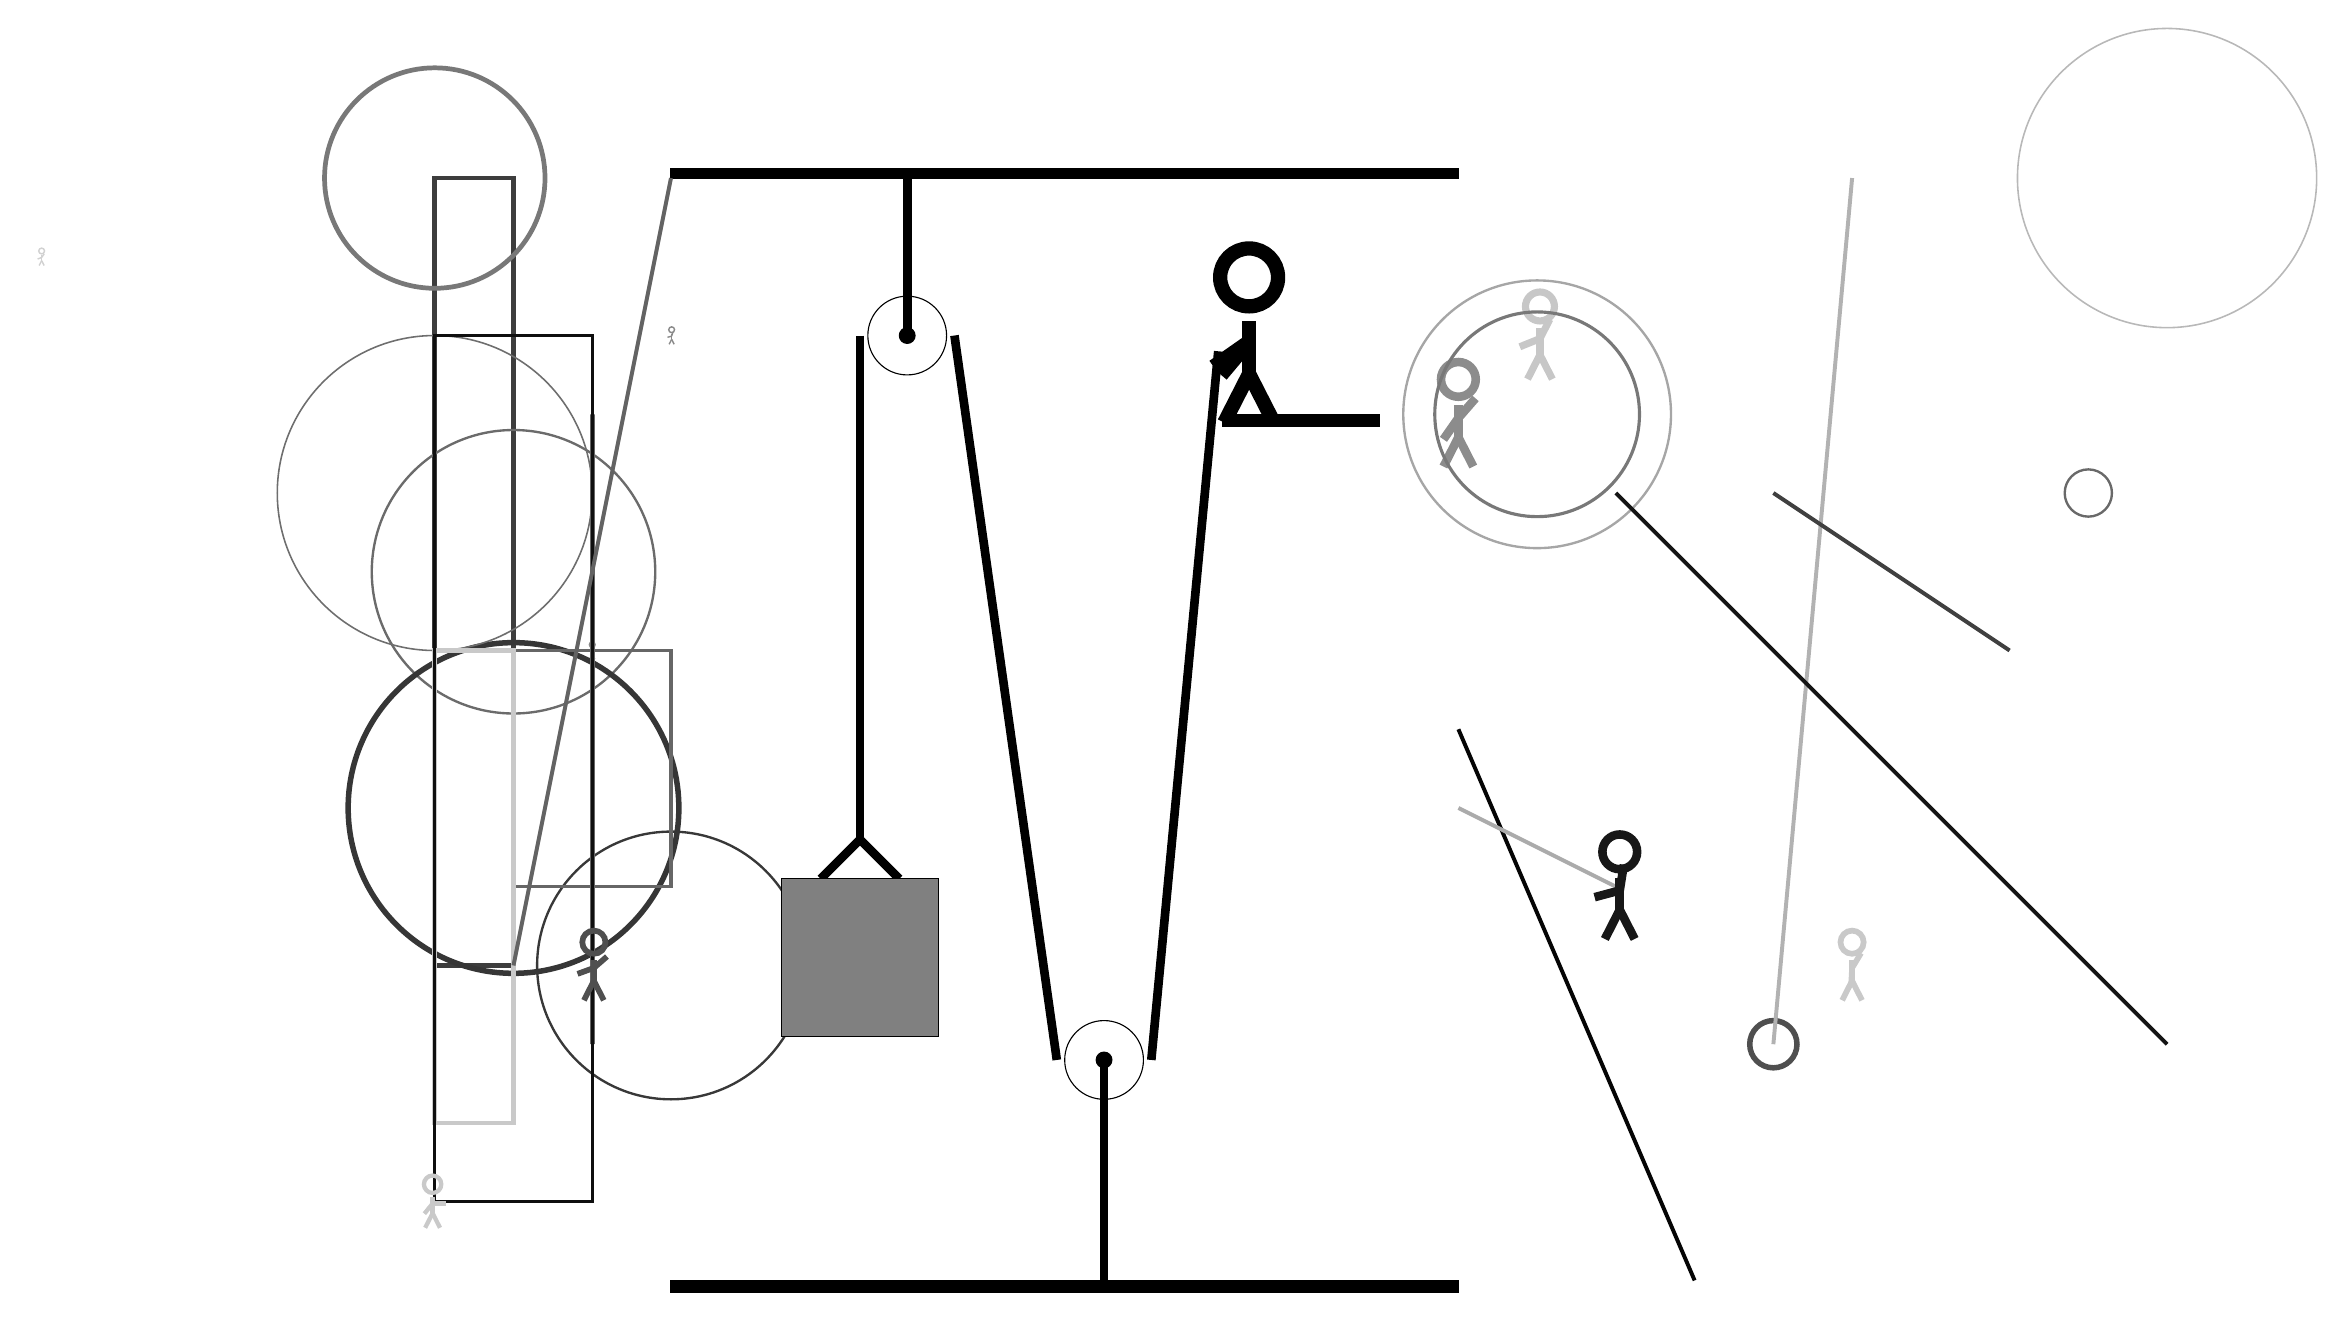
\begin{tikzpicture}
			%%%%% START %%%%%
			
			\draw[fill=black] (-2, 14) rectangle (8, 14.125);
			
			\draw (3.5, 2.8) circle (0.5);
			\draw[fill=black] (3.5, 2.8) circle (0.1);
			\draw[line width=1.1mm] (3.5, 2.8) -- (3.5, 0);
			
			\draw (1, 12) circle (0.5);
			\draw[fill=black] (1, 12) circle (0.1);
			\draw[line width=1.1mm] (1, 14) -- (1, 12);
			
			\draw [line width=0.7mm, color=black!69](12, 3) circle (0.3);
			
			\draw[line width=0.6mm, color=black!76] (-4, 4) rectangle (-5, 14);
			\draw [line width=0.3mm, color=black!78](-2, 4) circle (1.7);
			\node[line width=0.4mm, color=black!22] at (9, 12) {\Strichmaxerl[5][22][63]};
			\draw[line width=0.5mm, color=black!30](12, 3) -- (13, 14);
			\draw [line width=0.3mm, color=black!58](-4, 9) circle (1.8);
			\node[line width=0.7mm, color=black!46] at (-3, 8) {\Strichmaxerl[1][85][70]};
			
			\draw[line width=0.5mm, color=black!98](8, 7) -- (11, 0);
			\node[line width=0.2mm, color=black!45] at (8, 11) {\Strichmaxerl[6][55][49]};
			
			\draw[line width=0.2mm, color=black!97] (-3, 8) rectangle (-3, 9);
			\draw [line width=0.7mm, color=black!79](-4, 6) circle (2.1);
			\draw [line width=0.4mm, color=black!53](9, 11) circle (1.3);
			\draw[line width=0.5mm, color=black!33](8, 6) -- (10, 5);
			
			\draw [line width=0.2mm, color=black!57](-5, 10) circle (2.0);
			\draw[line width=0.5mm, color=black!75](12, 10) -- (15, 8);
			\node[line width=0.7mm, color=black!18] at (-10, 13) {\Strichmaxerl[1][22][54]};
			\draw[line width=0.4mm, color=black!60] (-4, 8) rectangle (-2, 5);
			
			\draw[line width=0.6mm, color=black!21] (-4, 8) rectangle (-5, 2);
			\draw[line width=0.6mm, color=black!60] (-3, 11) rectangle (-3, 3);
			\draw[line width=0.4mm, color=black!94] (-3, 1) rectangle (-5, 12);
			\draw[line width=0.5mm, color=black!61](-4, 4) -- (-2, 14);
			
			\draw[line width=0.5mm, color=black!37] (9, 9) rectangle (9, 9);
			
			\draw [line width=0.6mm, color=black!53](-5, 14) circle (1.4);
			\node[line width=0.3mm, color=black!46] at (-2, 12) {\Strichmaxerl[1][15][73]};
			\draw [line width=0.2mm, color=black!28](17, 14) circle (1.9);
			
			\node[line width=0.5mm, color=black!21] at (13, 4) {\Strichmaxerl[4][87][59]};
			\draw [line width=0.3mm, color=black!59](16, 10) circle (0.3);
			\node[line width=0.3mm, color=black!91] at (10, 5) {\Strichmaxerl[6][15][81]};
			
			\draw [line width=0.3mm, color=black!35](9, 11) circle (1.7);
			\node[line width=0.4mm, color=black!69] at (-3, 4) {\Strichmaxerl[4][20][41]};
			\draw[line width=0.5mm, color=black!92](10, 10) -- (17, 3);
			
			\node[line width=0.5mm, color=black!21] at (-5, 1) {\Strichmaxerl[3][51][0]};
			
			\draw[line width=1.1mm](-0.1, 5.1) --  (0.4, 5.6) -- (0.9, 5.1);
			\draw[fill=black!50] (-0.6, 5.1) rectangle (1.4, 3.1);
			
			\draw[line width=1.1mm](0.4, 12) -- (0.4, 5.6);
			\centerarc[line width=1.1mm](1, 12)(180:0:0.6)
			\draw[line width=1.1mm](1.6, 12) -- (2.9, 2.8);
			\centerarc[line width=1.1mm](3.5, 2.8)(180:360:0.6)
			\draw[line width=1.1mm](4.1, 2.8) -- (4.95, 11.8);
			
			\node at (5.3, 12) {\Strichmaxerl[10][35][-130]};
			\draw[fill=black] (5, 11) rectangle (7, 10.85);
			
			\draw[fill=black] (-2, 0) rectangle (8, -0.15);
			
			%%%%% END %%%%%
		\end{tikzpicture}
	\end{figure}	
\end{document}